\documentclass[aip,jcp,reprint,noshowkeys,superscriptaddress]{revtex4-1}
\usepackage{graphicx,dcolumn,bm,xcolor,microtype,multirow,amscd,amsmath,amssymb,amsfonts,physics,longtable,wrapfig}
\usepackage[version=4]{mhchem}
\usepackage{mathrsfs}
\allowdisplaybreaks[1]

\usepackage[utf8]{inputenc}
\usepackage[T1]{fontenc}
\usepackage{txfonts}

\usepackage[
    colorlinks,
    linkcolor={red!50!black},
    citecolor={red!70!black},
    urlcolor={red!80!black}
	]{hyperref}
\urlstyle{same}

\newcommand{\ie}{\textit{i.e.}}
\newcommand{\eg}{\textit{e.g.}}
\newcommand{\alert}[1]{\textcolor{red}{#1}}
\usepackage[normalem]{ulem}
\newcommand{\titou}[1]{\textcolor{red}{#1}}
\newcommand{\trashPFL}[1]{\textcolor{\red}{\sout{#1}}}
\newcommand{\PFL}[1]{\titou{(\underline{\bf PFL}: #1)}}

\newcommand{\cre}[1]{\Hat{a}_{#1}^{\dag}}
\newcommand{\ani}[1]{\Hat{a}_{#1}}
\newcommand{\ca}[2]{\Hat{a}^{#1}_{#2}}

\newcommand{\mc}{\multicolumn}
\newcommand{\fnm}{\footnotemark}
\newcommand{\fnt}{\footnotetext}
\newcommand{\tabc}[1]{\multicolumn{1}{c}{#1}}
\newcommand{\QP}{\textsc{quantum package}}
\newcommand{\T}[1]{#1^{\intercal}}

% coordinates
\newcommand{\br}{\boldsymbol{r}}
\newcommand{\bx}{\boldsymbol{x}}
\newcommand{\bI}{\boldsymbol{1}}
\newcommand{\cK}{\mathcal{K}}
\newcommand{\bG}{\boldsymbol{G}}
\newcommand{\bH}{\boldsymbol{H}}
\newcommand{\bM}{\boldsymbol{M}}
\newcommand{\bE}{\boldsymbol{E}}
\newcommand{\bSigma}{\boldsymbol{\Sigma}}
\newcommand{\bA}{\boldsymbol{A}}
\newcommand{\bB}{\boldsymbol{B}}
\newcommand{\bC}{\boldsymbol{C}}
\newcommand{\bD}{\boldsymbol{D}}
\newcommand{\bS}{\boldsymbol{S}}
\newcommand{\bN}{\boldsymbol{N}}
\newcommand{\bX}{\boldsymbol{X}}
\newcommand{\bY}{\boldsymbol{Y}}
\newcommand{\bZ}{\boldsymbol{Z}}
\newcommand{\bPi}{\boldsymbol{\Pi}}
\newcommand{\bcalM}{\boldsymbol{\mathcal M}}
\newcommand{\bcalS}{\boldsymbol{\mathcal S}}

% orbital energies
\newcommand{\eps}{\epsilon}
\newcommand{\irr}{\text{irr}}

% shortcuts for greek letters
\newcommand{\si}{\sigma}
\newcommand{\la}{\lambda}
\newcommand{\ii}{\mathrm{i}}
\newcommand{\up}{\uparrow}
\newcommand{\dw}{\downarrow}
\newcommand{\upup}{\up\up}
\newcommand{\updw}{\up\dw}
\newcommand{\dwup}{\dw\up}
\newcommand{\dwdw}{\dw\downarrow}

\newcommand{\h}{\text{1h}}
\newcommand{\p}{\text{1p}}
\newcommand{\hp}{\text{1h+1p}}
\newcommand{\hhp}{\text{2h1p}}
\newcommand{\pph}{\text{2p1h}}
\newcommand{\ph}{\text{ph}}
\newcommand{\eh}{\text{eh}}
\newcommand{\he}{\text{he}}
\newcommand{\ee}{\text{ee}}
\newcommand{\teh}{\overline{\text{eh}}}
\newcommand{\pp}{\text{pp}}
\newcommand{\hh}{\text{hh}}
\newcommand{\xc}{\text{xc}}

% this note
\newcommand{\Lag}{\mathcal{L}}
\newcommand{\sLag}{\bar{\mathcal L}}
\newcommand{\act}{\mathrm{act}}
\newcommand{\scv}{\text{cv}}
\newcommand{\sca}{\text{ca}}
\newcommand{\sav}{\text{av}}
\newcommand{\saa}{\text{aa}}
\newcommand{\svv}{\text{vv}}
\newcommand{\scc}{\text{cc}}

% addresses
\newcommand{\LCPQ}{Laboratoire de Chimie et Physique Quantiques (UMR 5626), Universit\'e de Toulouse, CNRS, UPS, France}

% statement-status markers used throughout the notes
\newcommand{\Exact}{\textbf{Exact identity.}\ }
\newcommand{\Established}{\textbf{Established result.}\ }
\newcommand{\Proposed}{\textbf{Proposed approximation.}\ }

\newcommand{\bt}{\boldsymbol{t}}
\newcommand{\bT}{\boldsymbol{T}}
\newcommand{\bW}{\boldsymbol{W}}
\newcommand{\bK}{\boldsymbol{K}}
\begin{document}

\title{Extended channel RPAs as a coupled-cluster-type amplitude equation on a CAS vacuum:\\ construction, energy functional and N$_2$ tests}

\begin{abstract}
The extended (ERPA) particle--hole, crossed particle--hole and particle--particle
problems of \texttt{erpa\_channels.tex} are combined into a single amplitude
equation following the common-amplitude construction of \texttt{Pa2CCD.tex}.
Each channel Riccati equation acquires the ERPA metric,
$\bB+\bA\,\bt\bN+\bN\bt\bA+\bN\bt\bB\bt\bN=0$ for the particle--hole channel,
the source and free terms are no longer channel independent and are replaced
by their fermionic antisymmetrization, and the amplitude space is the set of
Dyall-external doubles.  The correlation energy is
$E_c=\tfrac14\sum B_{(pq),(rs)}t^{pr}_{qs}$, with $B$ the exact coupling
$\langle\Psi_0|\hat H|\Phi\rangle$ to the doubly excited states.  For a
Hartree--Fock vacuum the equation is the non-mosaic CCD equation (verified
numerically).  N$_2$ tests show two things.  For doubles with at most one
active index the construction is quantitatively right: its second order
agrees with the corresponding SC-NEVPT2 classes to within $0.4$~mE$_h$ per
class along the whole 6-31G curve, and the combined
ring$+$crossed-ring$+$ladder equation lies within $6$--$16\%$ of an
exact-metric class-CI where one is available, whereas the ring channel alone
diverges and the ladder channel alone recovers about half.  For doubles with
two active indices the quasi-boson factorization of the doubles norm,
$(1-n_x)(1-n_y)$ instead of $1-n_x-n_y+\Gamma_{xy,xy}$, fails by factors up
to $50$ in N$_2$, and since these are the only external doubles of the
minimal-basis CAS(6,6) problem, the STO-3G dissociation curve is not
described by the quasi-boson equations; a brute-force treatment with exact
pair metrics recovers $98\%$ of $E_{\rm FCI}-E_{\rm CASSCF}$ and identifies the
$N\pm2$ pair-addition metric as the missing ingredient.
\end{abstract}

\maketitle

%%%%%%%%%%%%%%%%%%%%%%%%%
\section{Scope}
\label{sec:scope}
%%%%%%%%%%%%%%%%%%%%%%%%%

\texttt{Pa2CCD.tex} shows that the three static channel problems of the
fixed-kernel parquet model (direct electron--hole $\eh$, transverse $\teh$,
particle--particle $\pp$), built on a Hartree--Fock determinant, combine into
the non-mosaic CCD residual once (i) each channel is written as a Riccati
equation, (ii) all three channel amplitudes are arrangements of one
antisymmetric doubles tensor, and (iii) the common source and free term are
counted once while the antisymmetrized scattering terms are summed.
\texttt{erpa\_channels.tex} gives the three channel problems for an arbitrary
vacuum in terms of its 1- and 2-RDM, in the extended-RPA sense of
Refs.~\cite{Rowe1968,ChatterjeePernal2012}.  These notes carry out steps (i)--(iii)
for that extended setting (Secs.~\ref{sec:riccati}--\ref{sec:construction}),
define the energy functional (Sec.~\ref{sec:energy}), state where the
underlying quasi-boson approximation is exact and where it is not
(Sec.~\ref{sec:validity}), and test everything on N$_2$ with CASSCF
references (Sec.~\ref{sec:numerics}).  Notation is that of
\texttt{erpa\_channels.tex}: $i,j$ core, $a,b$ virtual, $x,y,z,w$ active and
$u,v$ active summation spin orbitals; $f$ the generalized Fock matrix, $\sLag$
the symmetrized Lagrangian, $\gamma$, $\Gamma$, $\lambda$ the 1-RDM, 2-RDM
and cumulant.  All quantities are real.  The implementation is
\texttt{numerics/erpa\_ccd/}.

%%%%%%%%%%%%%%%%%%%%%%%%%
\section{Channel Riccati equations with a metric}
\label{sec:riccati}
%%%%%%%%%%%%%%%%%%%%%%%%%

\subsection{Particle--hole channel}

\Exact Let $\mathcal E$ be the forward (excitation) manifold, $\bN$ the
positive ERPA metric and $\bA$, $\bB$ the matrices of
Eq.~(ph-AB) of \texttt{erpa\_channels.tex}, so that the channel problem is
\begin{widetext}
\begin{equation}
  \begin{pmatrix}\bA&\bB\\ \bB&\bA\end{pmatrix}
  \begin{pmatrix}\bX\\ \bY\end{pmatrix}
  =\begin{pmatrix}\bN&0\\0&-\bN\end{pmatrix}
  \begin{pmatrix}\bX\\ \bY\end{pmatrix}\boldsymbol\Omega ,
  \label{eq:ph-gen}
\end{equation}
\end{widetext}
with $\bX^{T}\bN\bX-\bY^{T}\bN\bY=\bI$
and $\bX$, $\bY$ collecting the positive-norm solutions.  Define
$\bT=\bY\bX^{-1}$ and $\bW=\bX\boldsymbol\Omega\bX^{-1}$.  The two block rows
read $\bA+\bB\bT=\bN\bW$ and $\bB+\bA\bT=-\bN\bT\bW$, and eliminating $\bW$
gives $\bB+\bA\bT+\bN\bT\bN^{-1}(\bA+\bB\bT)=0$.  With the
fermion-normalized amplitude
\begin{widetext}
\begin{equation}
  \bt=\bT\bN^{-1}=\bN^{-1/2}\bT_{s}\bN^{-1/2},\qquad
  \bT_s=\bY_s\bX_s^{-1},\quad \bX_s=\bN^{1/2}\bX,\ \bY_s=\bN^{1/2}\bY ,
  \label{eq:t-def}
\end{equation}
\end{widetext}
which is symmetric because the boson-normalized $\bT_s$ is, the Riccati
equation becomes
\begin{equation}
  \bB+\bA\,\bt\,\bN+\bN\,\bt\,\bA+\bN\,\bt\,\bB\,\bt\,\bN=0 .
  \label{eq:riccati-ph}
\end{equation}
Equation~\eqref{eq:t-def} is the quasi-boson statement
$\hat Q_\nu|\Psi\rangle=0$ for
$|\Psi\rangle\propto\exp\bigl(\tfrac12\sum t_{(pq),(rs)}\hat E_{pq}\hat E_{rs}\bigr)|\Psi_0\rangle$
with the bosons $\hat b^\dagger_{pq}=N_{pq}^{-1/2}\hat E_{pq}$, $[\hat b_{pq},\hat b^\dagger_{rs}]\simeq\delta\delta$;
the metric factors in Eq.~\eqref{eq:riccati-ph} are the only trace of the
correlated vacuum in the structure of the equation.  For a Hartree--Fock
vacuum $\bN=\bI$ and Eq.~\eqref{eq:riccati-ph} is the direct-channel Riccati
equation of \texttt{Pa2CCD.tex}.  The plasmon identity
$\sum_\nu\omega_\nu-\mathrm{Tr}\,\bN^{-1/2}\bA\bN^{-1/2}=\mathrm{Tr}(\bB\bt)$
holds unchanged.

\subsection{Crossed particle--hole channel}

\Established With $\bB\to-\bB$ [Eq.~(teh-erpa) of \texttt{erpa\_channels.tex}]
the Riccati equation is
$-\bB+\bA\bt'\bN+\bN\bt'\bA-\bN\bt'\bB\bt'\bN=0$, which is solved by
$\bt'=-\bt$.  As arrays over (hole, particle) pairs the crossed amplitude is
minus the direct one, exactly as $J_{\teh}$ of \texttt{Pa2CCD.tex} prescribes
($T^{\teh}_{ib,ja}=t^{ab}_{ij}=-T^{\eh}_{ib,ja}$); the channels differ in how
the array is attached to the fermionic tensor, not in the array itself.

\subsection{Particle--particle channel}

\Exact With the particle-like and hole-like pair sectors $\mathcal P$,
$\mathcal H$, metrics $\bN_{\mathcal P},\bN_{\mathcal H}>0$ and the blocks
$\bA^{\pp}$, $\bB^{\pp}$, $\bC^{\pp}$ of Eq.~(pp-ABC) of
\texttt{erpa\_channels.tex}, the same elimination applied to Eq.~(pp-rpa)
there, with $\bT=\bY\bX^{-1}$ (hole-pair rows, particle-pair columns) and
$\bt=\bT\bN_{\mathcal P}^{-1}$, gives
\begin{widetext}
\begin{equation}
  \bB^{\pp T}+\bC^{\pp}\,\bt\,\bN_{\mathcal P}+\bN_{\mathcal H}\,\bt\,\bA^{\pp}
  +\bN_{\mathcal H}\,\bt\,\bB^{\pp}\,\bt\,\bN_{\mathcal P}=0 ,
  \label{eq:riccati-pp}
\end{equation}
\end{widetext}
which for a Hartree--Fock vacuum is the particle--particle Riccati equation
of \texttt{Pa2CCD.tex} [its $\bD\to\bC^{\pp}$, $\bC\to\bA^{\pp}$].  With
unrestricted pair labels every pair contraction carries the factor $1/2$ of
its Eq.~(pair\_product).

%%%%%%%%%%%%%%%%%%%%%%%%%
\section{Common-amplitude construction on a correlated vacuum}
\label{sec:construction}
%%%%%%%%%%%%%%%%%%%%%%%%%

\subsection{Fermionic doubles tensor and amplitude space}
\label{sec:space}

\Proposed The common object is a fermionic doubles tensor $t^{pr}_{qs}$ with
$p,r$ particle-like (virtual or active) and $q,s$ hole-like (core or active),
antisymmetric under $p\leftrightarrow r$ and $q\leftrightarrow s$, and the
channel amplitudes are its arrangements,
\begin{equation}
  T^{\eh}_{(pq),(rs)}=t^{pr}_{qs},\qquad
  T^{\teh}_{(ps),(rq)}=t^{pr}_{qs},\qquad
  T^{\pp}_{(qs),(pr)}=t^{pr}_{qs} .
  \label{eq:J-ext}
\end{equation}
The Dyall partition of \texttt{mr-hedin.tex} and Ref.~\cite{WangFangLi2026} fixes the amplitude space: the
residual interaction has no all-active elements, all-active single and pair
excitations belong to the reference, and the quasi-boson metric is exact
only for pairs with an inactive index (Sec.~\ref{sec:validity}).  We
therefore keep the single-excitation manifold
$\mathcal E_{\rm in}=\{(ai),(xi),(ax)\}$ and the pair manifolds
$\mathcal P_{\rm in}=\{(ab),(ax)\}$, $\mathcal H_{\rm in}=\{(ij),(ix)\}$, and
define the external doubles space
\begin{equation}
  \mathscr D_{\rm ext}=\bigl\{t^{pr}_{qs}:\ (pq),(rs),(ps),(rq)\in\mathcal E_{\rm in}\bigr\},
  \label{eq:Dext}
\end{equation}
so that both electron--hole arrangements exist for every element; the
particle--particle arrangement exists when in addition
$(pr)\in\mathcal P_{\rm in}$ and $(qs)\in\mathcal H_{\rm in}$.  In the
language of NEVPT2 classes this retains
\begin{center}
\begin{tabular}{llll}
class & excitation & NEVPT2 label & channels\\\hline
$(\scv,\scv)$ & $ij\to ab$ & $S_{ijrs}(0)$ & $\eh,\teh,\pp$\\
$(\scv,\sca)$ & $ij\to ax$ & $S_{ijr}(+1)$ & $\eh,\teh,\pp$\\
$(\scv,\sav)$ & $ix\to ab$ & $S_{rsi}(-1)$ & $\eh,\teh,\pp$\\
$(\sca,\sca)$ & $ij\to xy$ & $S_{ij}(+2)$ & $\eh,\teh$\\
$(\sav,\sav)$ & $xy\to ab$ & $S_{rs}(-2)$ & $\eh,\teh$
\end{tabular}
\end{center}
and leaves out $(\sca,\sav)$ [$ix\to ay$, $S_{ir}(0)'$], whose crossed
arrangement is the all-active pair $(xy)$, and the semi-internal classes
$(\sca,\saa)$, $(\sav,\saa)$ [$S_{i}(+1)'$, $S_{r}(-1)'$], which contain an
all-active boson.  For $(\sca,\sca)$ and $(\sav,\sav)$ the pp arrangement
would require the all-active pairs $(xy)$, whose commutator metric
$1-n_x-n_y$ is not a norm; these classes carry no ladder term.

\subsection{One-body and two-body parts}

\Proposed As in \texttt{Pa2CCD.tex} the channel matrices are split into a
free (one-body) part and a kernel.  From the cumulant forms of
\texttt{erpa\_channels.tex},
\begin{widetext}
\begin{align}
  A^{0}_{(pq),(rs)}&=\gamma_{qs}f_{pr}+\gamma_{pr}f_{qs}-\delta_{pr}\sLag_{qs}-\delta_{qs}\sLag_{pr},
  \qquad \bK=\bA-\bA^{0},
  \label{eq:A0}\\
  M^{\pp,0}_{(pq),(rs)}&=P(pq)P(rs)\bigl[\delta_{qs}(f-\sLag)_{pr}-\gamma_{qs}f_{pr}\bigr],
  \qquad \bK^{\pp}_{\mathcal{PP}}=\bA^{\pp}-\bA^{\pp,0},\ \ \bK^{\pp}_{\mathcal{HH}}=\bC^{\pp}-\bC^{\pp,0},
  \label{eq:A0pp}
\end{align}
\end{widetext}
where $\bA^{0}$ reduces to $\delta_{ij}f_{ab}-\delta_{ab}f_{ij}$ in the
$\scv$--$\scv$ block and to $\delta_{ij}(f-\sLag)_{xy}-(\delta_{xy}-\gamma_{xy})f_{ij}$
in the $\sca$--$\sca$ block, \ie\ to the $N{\pm}1$ extended-Koopmans
matrices of the active space shifted by the core or virtual orbital
energies.  The kernels contain the integral terms with one or two active
densities and the cumulant.

\subsection{Sources and free terms are not channel independent}

\Exact Two features are new relative to the Hartree--Fock case.  First, the
sources differ: $B_{(pq),(rs)}=\langle\Psi_0|[[\hat H,\hat E_{pq}],\hat E_{rs}]|\Psi_0\rangle=\langle\Psi_0|\hat H\hat E_{pq}\hat E_{rs}|\Psi_0\rangle$
is the exact coupling to the doubly excited state, whereas the
particle--particle source is a different commutator; for $ij\to xy$,
\begin{widetext}
\begin{equation}
  B_{(xi),(yj)}-B^{\pp}_{(xy),(ij)}=\tfrac12\sum_{uv}\langle uv||ij\rangle\,\Gamma_{uv,xy}
  \label{eq:source-diff}
\end{equation}
\end{widetext}
[blocks (ph-B-ca-ca) and (pp-aa-cc) of \texttt{erpa\_channels.tex}].
Second, the free terms differ between the direct and the crossed arrangement,
because the metric factors in $\bA^0\bt\bN+\bN\bt\bA^0$ attach to different
pairs ($N_{(rs)}$ versus $N_{(rq)}$).  Both features disappear for
$\bN=\bI$, $\lambda=0$.

\Proposed The resolution is already implicit in the antisymmetrization maps
$U_\alpha$ of \texttt{Pa2CCD.tex}.  Write the channel residuals and their
common/scattering parts in the fermionic arrangement,
\begin{widetext}
\begin{align}
  \mathcal R^{\eh}[\bt]&=\bB+\bA\bt\bN+\bN\bt\bA+\bN\bt\bB\bt\bN ,
  &\mathcal C^{\eh}[\bt]&=\bB+\bA^{0}\bt\bN+\bN\bt\bA^{0},
  &\chi^{\eh}&=\mathcal R^{\eh}-\mathcal C^{\eh},
  \nonumber\\
  \mathcal R^{\teh}[\bt]&=-\bB+\bA\bt'\bN+\bN\bt'\bA-\bN\bt'\bB\bt'\bN ,
  &\mathcal C^{\teh}[\bt]&=-\bB+\bA^{0}\bt'\bN+\bN\bt'\bA^{0},
  &\chi^{\teh}&=\mathcal R^{\teh}-\mathcal C^{\teh},
  \nonumber\\
  \chi^{\pp}[\bt]&=\bK^{\pp}_{\mathcal{HH}}\bt\bN_{\mathcal P}+\bN_{\mathcal H}\bt\bK^{\pp}_{\mathcal{PP}}+\bN_{\mathcal H}\bt\bB^{\pp}\bt\bN_{\mathcal P},
  \label{eq:pieces}
\end{align}
\end{widetext}
with $\bt$ the direct and $\bt'$ the crossed arrangement of the same tensor.
Because $\bt$ evaluated at the crossed pairing equals $-\bt'$, the direct
common term evaluated at the crossed pairing equals $-\mathcal C^{\teh}$, and
likewise $\chi^{\eh}\to-\chi^{\teh}$; hence the fermionic antisymmetrization
gives $U[\mathcal C^{\eh}]=\tfrac12(\mathcal C^{\eh}+\mathcal C^{\teh})$ and
$U[\chi^{\eh}]=U[\chi^{\teh}]=\tfrac12(\chi^{\eh}+\chi^{\teh})$, the extended
form of Eqs.~(projected\_eh\_identity)--(projected\_channel\_identity) of
\texttt{Pa2CCD.tex}.  Retaining the (antisymmetrized) common term once and
adding the three antisymmetrized scattering terms, the combined doubles
equation is
\begin{widetext}
\begin{equation}
  \boxed{\;
  \mathcal R[\bt]=\tfrac12\bigl(\mathcal C^{\eh}+\mathcal C^{\teh}\bigr)
  +\bigl(\chi^{\eh}+\chi^{\teh}\bigr)+\chi^{\pp}
  =\mathcal R^{\eh}+\mathcal R^{\teh}-\tfrac12\bigl(\mathcal C^{\eh}+\mathcal C^{\teh}\bigr)+\chi^{\pp}=0
  \quad\text{on }\mathscr D_{\rm ext}.\;}
  \label{eq:combined}
\end{equation}
\end{widetext}
$\mathcal R[\bt]$ is antisymmetric in $p\leftrightarrow r$ and
$q\leftrightarrow s$ by construction; the particle--particle source is not
counted (it is the common term's job) and enters only through the quadratic
ladder term.  Dropping $\chi^{\pp}$ gives the ring$+$crossed-ring equation,
dropping $\chi^{\eh}+\chi^{\teh}$ the ladder equation, dropping both the
second-order (linear) equation.

\Exact \emph{Hartree--Fock limit.}  For a determinant,
Eq.~\eqref{eq:combined} is Eq.~(residual\_channel\_sum) of
\texttt{Pa2CCD.tex} and therefore the non-mosaic CCD residual.  This was
checked numerically (\texttt{test\_hf\_limit.py}, N$_2$/STO-3G): for a
random antisymmetric $\bt$ the combined residual and an independent
implementation of Eq.~(nonmosaic\_ccd) agree to $4\times10^{-14}$, the
channel matrices equal the RPA and pp-RPA blocks, and the second-order
solution gives the MP2 energy.

\subsection{Energy functional}
\label{sec:energy}

\Proposed The correlation energy is evaluated with the CCD-type functional
\begin{widetext}
\begin{equation}
  E_c=\frac14\sum_{t^{pr}_{qs}\in\mathscr D_{\rm ext}}B_{(pq),(rs)}\,t^{pr}_{qs},
  \qquad B_{(pq),(rs)}=\langle\Psi_0|\hat H\hat E_{pq}\hat E_{rs}|\Psi_0\rangle ,
  \label{eq:Ec}
\end{equation}
\end{widetext}
where $B$ is fermionic-antisymmetric on $\mathscr D_{\rm ext}$
($B_{(ps),(rq)}=-B_{(pq),(rs)}$, checked to $10^{-15}$).  Three reasons.
(i)~For a determinant it is $\tfrac14\sum\langle ij||ab\rangle t^{ab}_{ij}$.
(ii)~With the common term alone, $t^{(1)}=-B/[N_{pq}N_{rs}(\omega_{pq}+\omega_{rs})]$
for diagonal $\bA^0$ ($\omega=A^0/N$), and Eq.~\eqref{eq:Ec} is the
second-order energy of the internally contracted doubles with norm
$N_{pq}N_{rs}$ and excitation energy $\omega_{pq}+\omega_{rs}$, each
fermionic double counted once.  (iii)~The plasmon formula $\tfrac12\mathrm{Tr}(\bB\bt)$
of the single channel is twice Eq.~\eqref{eq:Ec} and double counts
second-order exchange, which is why \texttt{Pa2CCD.tex} assigns one half of
the ring$+$crossed-ring terms to each electron--hole channel.  Singles are
absent because the CASSCF vacuum satisfies the generalized Brillouin
condition, Eq.~(brillouin) of \texttt{erpa\_channels.tex}.

%%%%%%%%%%%%%%%%%%%%%%%%%
\section{Where the quasi-boson construction is exact and where it is not}
\label{sec:validity}
%%%%%%%%%%%%%%%%%%%%%%%%%

\Exact For a single excitation with an inactive index the de-excitation
state vanishes ($\hat E_{ix}|\Psi_0\rangle=\hat E_{xa}|\Psi_0\rangle=0$), so
\begin{widetext}
\begin{equation}
  \langle[\hat E_{qp},[\hat H,\hat E_{rs}]]\rangle
  =\langle\Phi_{pq}|\hat H-E_0|\Phi_{rs}\rangle ,\qquad
  \langle[\hat E_{qp},\hat E_{rs}]\rangle=\langle\Phi_{pq}|\Phi_{rs}\rangle,
  \qquad |\Phi_{pq}\rangle=\hat E_{pq}|\Psi_0\rangle ,
  \label{eq:tda-exact}
\end{equation}
\end{widetext}
\ie\ the ERPA blocks of $\mathcal E_{\rm in}$ are the exact Hamiltonian and
overlap matrices of the singly excited states (the $N{\pm}1$ EKT problems of
the active space shifted by the inactive orbital energy).  The
approximation of Sec.~\ref{sec:construction} is therefore entirely in the
treatment of the \emph{doubles}, where the quasi-boson ansatz replaces the
norm of $\hat E_{pq}\hat E_{rs}|\Psi_0\rangle$ by $N_{pq}N_{rs}$.  This is
exact whenever one of the two excitations is a core$\to$virtual excitation,
because that boson is uncorrelated with the active space; hence it is exact
for $(\scv,\scv)$, $(\scv,\sca)$ and $(\scv,\sav)$.  For two active indices
it is not:
\begin{widetext}
\begin{align}
  \langle\Psi_0|\hat E_{jy}\hat E_{ix}\hat E_{xi}\hat E_{yj}|\Psi_0\rangle
  &=\langle\ani{y}\ani{x}\cre{x}\cre{y}\rangle=1-n_x-n_y+\Gamma_{xy,xy}
  =(1-n_x)(1-n_y)+\lambda_{xy,xy},
  \label{eq:norm-caca}\\
  \langle\Psi_0|\hat E_{yb}\hat E_{xa}\hat E_{ax}\hat E_{by}|\Psi_0\rangle
  &=\Gamma_{xy,xy}=n_xn_y+\lambda_{xy,xy}
  \label{eq:norm-avav}
\end{align}
\end{widetext}
(natural spin orbitals).  For nearly doubly occupied or nearly empty active
orbitals the product $N_{pq}N_{rs}$ is tiny while the cumulant term is not,
and the ratio of exact to quasi-boson norm reaches $50$ for N$_2$ at
$0.9$~\AA\ (Table~\ref{tab:sto3g}); the second-order energy, whose
denominators carry $N_{pq}N_{rs}$, is overestimated by the same factors.  The
particle--particle commutator metric does not cure this: it is the
difference $\mathcal N^{+}-\mathcal N^{-}$ of the pair-addition and
pair-removal overlaps, $\mathcal N^{+}_{(xy),(zw)}=\langle\ani{y}\ani{x}\cre{z}\cre{w}\rangle=S^{\pp}_{(xy),(zw)}+\Gamma_{zw,xy}$,
and vanishes for half-filled pairs.  The correct object for
$ij\to xy$ is $\mathcal N^{+}$ alone (and $\mathcal N^{-}$ for $xy\to ab$):
the active part of such a double is an $N{+}2$ (or $N{-}2$) pair-EKT state,
not a product of two $N{\pm}1$ bosons.  Replacing the two single-excitation
bosons by one pair boson with metric $\mathcal N^{\pm}$ and the corresponding
pair Hamiltonian is the consistent extension; it is not carried out here,
but Sec.~\ref{sec:numerics} shows by a brute-force calculation what it would
deliver.

%%%%%%%%%%%%%%%%%%%%%%%%%
\section{Numerical tests on N$_2$}
\label{sec:numerics}
%%%%%%%%%%%%%%%%%%%%%%%%%

\subsection{Setup}

PySCF~2.13; CASSCF with natural active orbitals and canonical core/virtual
orbitals; spin-orbital 1- and 2-RDM of the CASSCF vacuum assembled in the
full orbital space (antisymmetry, trace and energy checked to $10^{-13}$);
ERPA arrays from the formulas of \texttt{erpa\_channels.tex};
Eq.~\eqref{eq:combined} solved by DIIS with the diagonal of the common term
as preconditioner, to $|\mathcal R|<10^{-8}$.  References: FCI where
possible, SC-NEVPT2 (class resolved), and a brute-force exact-metric
treatment of individual doubles classes: the states $\hat E\hat E|\Psi_0\rangle$
are built explicitly in the full determinant space, their exact overlap
$\mathcal S$, Hamiltonian block $\mathcal H$ and coupling
$v=\langle\Phi|\hat H|\Psi_0\rangle$ are formed, and
$E_2=-v^{T}(\mathcal H-E_0\mathcal S)^{-1}v$ (second order with the full
Hamiltonian in the doubles block) and the class-CI energy (diagonalization
in $\{\Psi_0\}\oplus\{\Phi\}$) are evaluated after canonical
orthogonalization (\texttt{class\_exact.py}).

\subsection{STO-3G, CASSCF(6,6): only two-active-index doubles}

With the valence $\pi$/$\sigma$ CAS(6,6) and the $1s$, $2s$ orbitals
inactive, the minimal basis has no virtual orbitals; the external doubles
are $ij\to xy$ (retained, class $S_{ij}(+2)$) and the semi-internal
$i\to x$, $w\to z$ (excluded).  Table~\ref{tab:sto3g} and
Fig.~\ref{fig:sto3g} summarize the curve.

\begin{table*}[t]
\caption{N$_2$/STO-3G, CASSCF(6,6) vacuum.  Energies relative to CASSCF in
mE$_h$.  ``exact-metric'' is the brute-force second order with exact
overlaps and the full Hamiltonian in the doubles block, for the $ij\to xy$
class, the semi-internal class and both together; ``class-CI'' the CI in
the span of both classes.  ``quasi-boson'' are the solutions of
Eq.~\eqref{eq:combined} (second order and ring$+$crossed ring; the ladder
channel is empty) and the pure ERPA ring eigen-solution with
$\tfrac14\mathrm{Tr}(\bB\bt)$; $\dagger$: not converged.  The last column is
the largest ratio of the exact norm \eqref{eq:norm-caca} to
$(1-n_x)(1-n_y)$ over the nonvanishing $ij\to xy$ doubles.}
\label{tab:sto3g}
\small
\begin{ruledtabular}
\begin{tabular}{cccccccccccccc}
$R$/\AA & $E_{\rm CASSCF}$/E$_h$ & FCI & NEVPT2 & $S_{ij}(+2)$ & $S_i(+1)'$ & E$_2^{\rm ex}(ij{\to}xy)$ & E$_2^{\rm ex}$(semi) & E$_2^{\rm ex}$(both) & class-CI & qb 2nd & qb ring$+$cr & ERPA ring & norm ratio\\
\hline
0.90 & $-107.277771$ & $-15.30$ & $-8.46$ & $-6.26$ & $-2.20$ & $-12.11$ & $-2.56$ & $-15.19$ & $-15.06$ & $-245.1$ & $-402.2^\dagger$ & $-316.2$ & 52.6\\
1.00 & $-107.533612$ & $-15.69$ & $-8.61$ & $-6.24$ & $-2.37$ & $-12.17$ & $-2.82$ & $-15.52$ & $-15.37$ & $-183.4$ & $-368.1^\dagger$ & $-241.7$ & 38.9\\
1.10 & $-107.638233$ & $-15.89$ & $-8.62$ & $-6.14$ & $-2.48$ & $-12.09$ & $-3.03$ & $-15.65$ & $-15.50$ & $-140.4$ & $-294.6$ & $-188.9$ & 29.7\\
1.20 & $-107.661519$ & $-15.82$ & $-8.50$ & $-5.96$ & $-2.53$ & $-11.82$ & $-3.16$ & $-15.51$ & $-15.35$ & $-108.7$ & $-246.4$ & $-149.1$ & 23.3\\
1.30 & $-107.644001$ & $-15.37$ & $-8.18$ & $-5.68$ & $-2.49$ & $-11.30$ & $-3.19$ & $-14.98$ & $-14.83$ & $-83.9$ & $-204.9^\dagger$ & $-117.3$ & 18.9\\
1.40 & $-107.608767$ & $-14.41$ & $-7.61$ & $-5.27$ & $-2.34$ & $-10.46$ & $-3.07$ & $-13.95$ & $-13.82$ & $-63.6$ & $-167.6$ & $-90.6$ & 15.6\\
1.60 & $-107.531396$ & $-10.69$ & $-5.63$ & $-3.94$ & $-1.69$ & $-7.72$ & $-2.27$ & $-10.20$ & $-10.12$ & $-32.2$ & $-99.6$ & $-47.6$ & 10.2\\
1.80 & $-107.477475$ & $-5.98$ & $-3.27$ & $-2.34$ & $-0.93$ & $-4.46$ & $-1.24$ & $-5.70$ & $-5.67$ & $-12.9$ & $-46.6$ & $-19.7$ & 5.3\\
2.00 & $-107.452262$ & $-2.89$ & $-1.66$ & $-1.20$ & $-0.46$ & $-2.24$ & $-0.62$ & $-2.79$ & $-2.79$ & $-4.8$ & $-19.1$ & $-7.5$ & 2.9\\
2.40 & $-107.440626$ & $-0.68$ & $-0.39$ & $-0.30$ & $-0.09$ & $-0.58$ & $-0.11$ & $-0.67$ & $-0.67$ & $-0.9$ & $-3.3^\dagger$ & $-1.4$ & 1.7\\
3.00 & $-107.437422$ & $-1.00$ & $-0.02$ & $-0.02$ & $-0.00$ & $-0.06$ & $-0.00$ & $-0.06$ & $-0.06$ & $-0.0$ & $-0.3^\dagger$ & $-0.1$ & 1.2\\
\end{tabular}
\end{ruledtabular}
\end{table*}

\begin{figure*}[t]
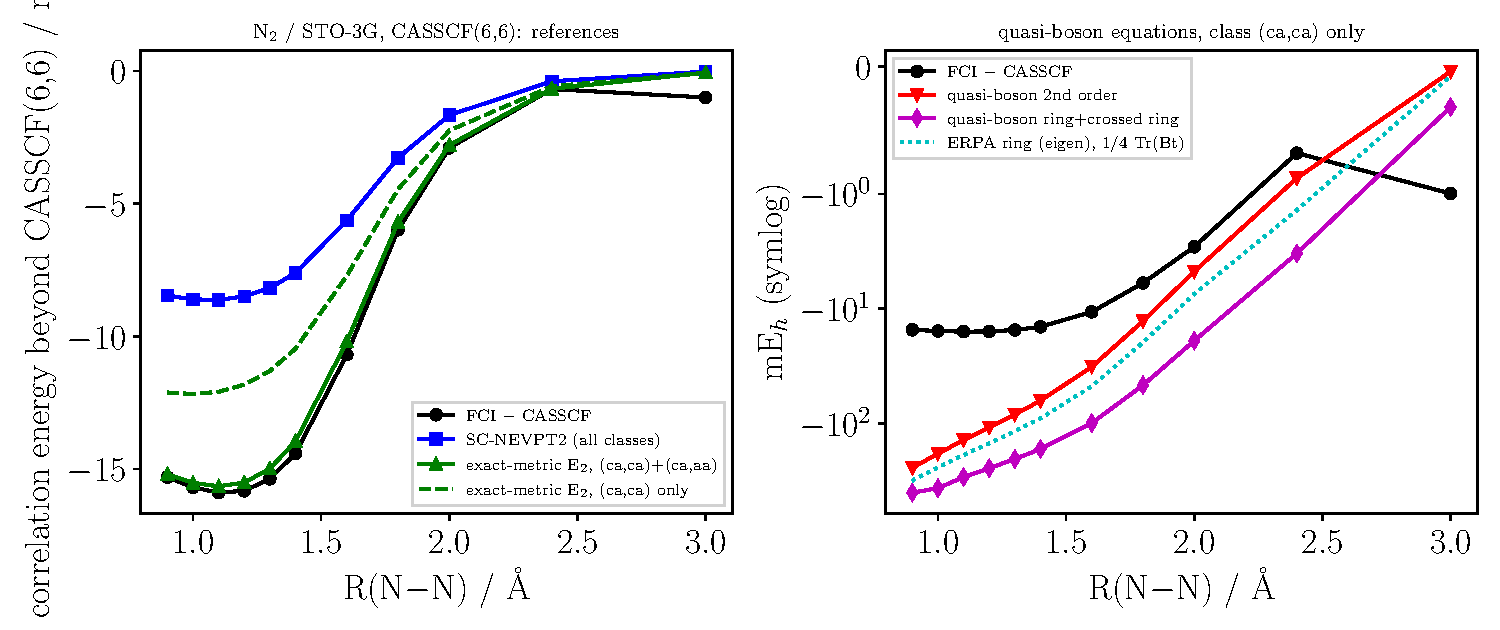
\includegraphics[width=0.95\textwidth]{erpa_ccd_n2_sto3g.pdf}
\caption{N$_2$/STO-3G, CASSCF(6,6) vacuum.  Left: FCI, SC-NEVPT2 and the
exact-metric second order of the external doubles classes relative to
CASSCF.  Right (symmetric log scale): the quasi-boson equations for the
$ij\to xy$ class.}
\label{fig:sto3g}
\end{figure*}

Three observations.  (i)~The exact-metric treatment of the two external
classes accounts for $98$--$99\%$ of $E_{\rm FCI}-E_{\rm CASSCF}$ for
$R\le2.4$~\AA, and second order with the full Hamiltonian in the doubles
block is within $0.2$~mE$_h$ of the class-CI: the external correlation is
weak and perturbative, and $ij\to xy$ carries $80\%$ of it.  (SC-NEVPT2
recovers about half, because it uses the Dyall Hamiltonian instead of the
full one inside the doubles block.)  (ii)~The quasi-boson equations fail by
an order of magnitude at short bond lengths and recover only when the
occupations approach $1/2$ at dissociation, exactly following the norm ratio
of the last column; this is the failure anticipated in
Sec.~\ref{sec:validity}, not an instability of the ring summation (the
second-order equation already fails).  (iii)~At $3$~\AA\ the remaining
$1$~mE$_h$ of FCI$-$CASSCF is outside both doubles classes (it belongs to
excitations with an active rearrangement accompanied by core$\to$active
singles, which become important when the inactive $2s$ orbitals mix with the
half-filled $2p$ shell).  In the minimal basis the quasi-boson common-amplitude
construction therefore cannot describe the dissociation curve, for a reason
that has nothing to do with the channel combination.

\subsection{STO-3G, $\sigma$-CASSCF(2,2): exact reference for the one-active-index classes}

To test the construction where its doubles norms are exact, the active space
is reduced to the $3\sigma_g$, $3\sigma_u$ pair, leaving the $\pi_g$
virtuals, so that the classes $ij\to ab$, $ij\to ax$ and $ix\to ab$ exist and
FCI and the brute-force class energies are available.  This reference
describes the $\pi$ bonds at the mean-field level, so the external
correlation is strong and grows quickly with $R$; the ring-containing
equations stop converging beyond $1.1$~\AA\ (the pure ERPA ring problem
acquires complex frequencies), and Table~\ref{tab:cas22} lists the three
geometries where all variants converge.

\begin{table*}[t]
\caption{N$_2$/STO-3G, $\sigma$-CASSCF(2,2) vacuum, doubles with at most one
active index; mE$_h$ relative to CASSCF.  The second-order energies are given
per class (quasi-boson and SC-NEVPT2) and for the exact-metric treatment;
``all'' refers to the three classes together.}
\label{tab:cas22}
\footnotesize
\begin{ruledtabular}
\begin{tabular}{cc ccc ccc ccc c cccc}
& & \multicolumn{3}{c}{quasi-boson 2nd order} & \multicolumn{3}{c}{SC-NEVPT2} & \multicolumn{3}{c}{exact-metric E$_2$} & class-CI & \multicolumn{4}{c}{Eq.~\eqref{eq:combined}, all classes}\\
$R$/\AA & FCI & $ij{\to}ab$ & $ij{\to}ax$ & $ix{\to}ab$ & $S_{ijrs}$ & $S_{ijr}$ & $S_{rsi}$ & $ij{\to}ab$ & $ij{\to}ax$ & all & all & 2nd & ring$+$cr & ladder & all\\
\hline
0.90 & $-101.49$ & $-63.30$ & $-1.87$ & $-0.10$ & $-63.05$ & $-1.87$ & $-0.03$ & $-76.44$ & $-2.45$ & $-80.38$ & $-77.11$ & $-65.28$ & $-219.6^\dagger$ & $-42.08$ & $-84.98$\\
1.00 & $-123.72$ & $-79.22$ & $-1.94$ & $-0.07$ & $-78.98$ & $-1.94$ & $-0.02$ & $-94.45$ & $-2.64$ & $-98.91$ & $-93.42$ & $-81.24$ & $-256.3^\dagger$ & $-50.55$ & $-107.97$\\
1.10 & $-149.36$ & $-98.99$ & $-2.00$ & $-0.07$ & $-98.75$ & $-2.00$ & $-0.02$ & $-116.11$ & $-2.82$ & $-121.23$ & $-112.09$ & $-101.07$ & $-108.9^\dagger$ & $-60.53$ & $-140.59$\\
\end{tabular}
\end{ruledtabular}
\end{table*}

The quasi-boson second order reproduces the SC-NEVPT2 class $S_{ijr}(+1)$
to all printed digits and $S_{ijrs}(0)$ to $0.3$~mE$_h$ (the small
difference is the Dyall versus generalized Fock operator in the
core--virtual denominators), confirming that for these classes the common
term is the Dyall-partitioned second order with exact norms.  The
exact-metric $E_2$ is $20\%$ larger because it also contains the first-order
coupling inside the doubles block, \ie\ the linear ring and ladder terms.
The combined equation reproduces this: at $0.9$ and $1.0$~\AA\ it is within
$6$ and $9\%$ of the exact-metric $E_2$ and within $10$ and $16\%$ of the
class-CI, overshooting slightly as a non-mosaic CCD does.  The ring channel
alone (whose plasmon counterpart is the ERPA correlation energy) does not
converge and, where it does, overestimates by a factor $2$--$3$; the ladder
channel alone recovers $45$--$55\%$.

\subsection{6-31G, CASSCF(6,6): one-active-index classes along the curve}

With virtual orbitals present the three boson-exact classes carry
$26$--$37$~mE$_h$ of the $56$--$73$~mE$_h$ SC-NEVPT2 correlation energy.
Table~\ref{tab:631g} and Fig.~\ref{fig:631g} compare the four variants of
Eq.~\eqref{eq:combined}, restricted to these classes, with the sum of the
corresponding SC-NEVPT2 classes along the dissociation curve (no exact
reference is available).

\begin{table}[t]
\caption{N$_2$/6-31G, CASSCF(6,6) vacuum, doubles with at most one active
index ($90\,112$ amplitudes); mE$_h$ relative to CASSCF.  NEVPT2$_3$ is
$S_{ijrs}(0)+S_{ijr}(+1)+S_{rsi}(-1)$; all variants converged.}
\label{tab:631g}
\begin{ruledtabular}
\begin{tabular}{ccccccccc}
$R$/\AA & $E_{\rm CASSCF}$/E$_h$ & NEVPT2 & NEVPT2$_3$ & 2nd & ring$+$cr & ladder & all\\
\hline
0.90 & $-108.785261$ & $-64.56$ & $-25.77$ & $-26.74$ & $-63.01$ & $-20.16$ & $-33.10$\\
1.00 & $-108.961201$ & $-66.38$ & $-26.10$ & $-26.93$ & $-62.69$ & $-20.35$ & $-33.41$\\
1.10 & $-109.015944$ & $-67.76$ & $-26.34$ & $-27.02$ & $-62.39$ & $-20.48$ & $-33.62$\\
1.20 & $-109.008954$ & $-69.03$ & $-26.63$ & $-27.16$ & $-62.35$ & $-20.64$ & $-33.90$\\
1.30 & $-108.973966$ & $-70.27$ & $-27.04$ & $-27.44$ & $-62.78$ & $-20.89$ & $-34.38$\\
1.40 & $-108.929735$ & $-71.48$ & $-27.63$ & $-27.90$ & $-63.81$ & $-21.29$ & $-35.12$\\
1.60 & $-108.848229$ & $-72.86$ & $-29.37$ & $-29.44$ & $-67.80$ & $-22.55$ & $-37.56$\\
1.80 & $-108.796148$ & $-70.66$ & $-31.57$ & $-31.51$ & $-73.14$ & $-24.23$ & $-40.84$\\
2.00 & $-108.773492$ & $-65.35$ & $-33.47$ & $-33.32$ & $-77.78$ & $-25.70$ & $-43.70$\\
2.40 & $-108.764878$ & $-58.52$ & $-35.61$ & $-35.38$ & $-83.72$ & $-27.28$ & $-46.89$\\
3.00 & $-108.762429$ & $-56.19$ & $-36.71$ & $-36.45$ & $-87.54$ & $-28.06$ & $-48.55$\\
\end{tabular}
\end{ruledtabular}
\end{table}

\begin{figure}[t]
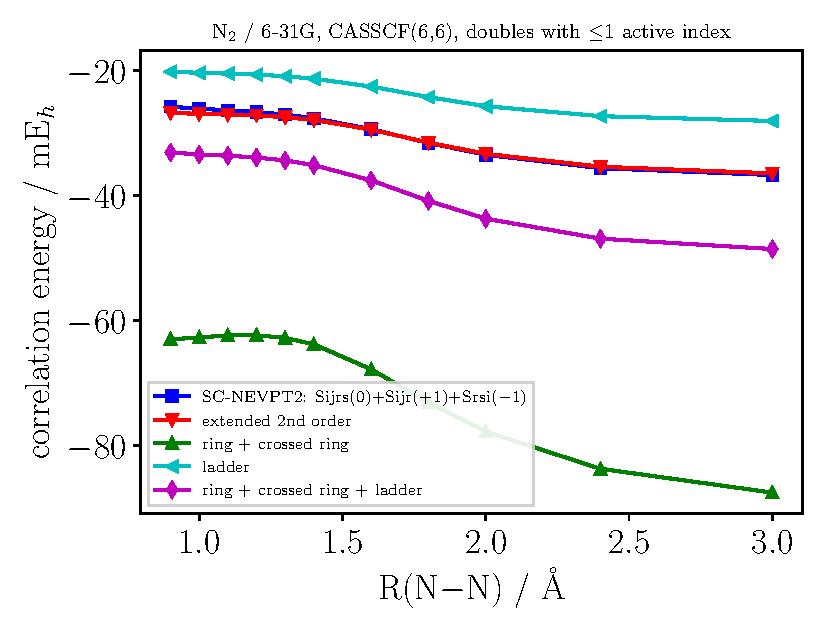
\includegraphics[width=0.95\columnwidth]{erpa_ccd_n2_631g.pdf}
\caption{N$_2$/6-31G, CASSCF(6,6) vacuum: the variants of
Eq.~\eqref{eq:combined} for the doubles with at most one active index,
compared with the sum of the corresponding SC-NEVPT2 classes.}
\label{fig:631g}
\end{figure}

The second-order energy follows NEVPT2$_3$ to better than $1$~mE$_h$ along
the whole curve (per class at $1.1$~\AA: $-8.71/-1.82/-16.49$ versus
$-8.35/-1.86/-16.13$~mE$_h$; at $2.0$~\AA: $-6.34/-3.37/-23.61$ versus
$-6.41/-3.48/-23.58$).  All channel-resummed variants converge at every
geometry with the CAS(6,6) vacuum, in contrast to the CAS(2,2) case: once
the static correlation is in the reference the external ring series is
stable.  The ordering is the same as in the exact-reference test, ring alone
$\approx2.4\times$ the second order, ladder alone $\approx0.76\times$, and
the combined equation $1.24$--$1.33\times$, which by the CAS(2,2) test is the
range of the exact-metric class energies.

\subsection{6-31G total-energy curves: RHF versus CASSCF(6,6) vacuum}

Figure~\ref{fig:totals} shows the same four variants as total energies,
once on the RHF determinant (no active space; the amplitude space is then
all $ij\to ab$ doubles and Eq.~\eqref{eq:combined} is non-mosaic CCD) and
once on the CASSCF(6,6) vacuum of Table~\ref{tab:631g}.  On the RHF vacuum
the ring$+$crossed-ring equation does not converge at any bond length, the
combined equation converges only up to $1.2$~\AA, the second order (MP2)
turns over and diverges towards dissociation ($-1.8$~E$_h$ at $3$~\AA), and
only the ladder equation converges everywhere, with a bounded but far too
small correlation energy at long range ($-0.69$~E$_h$ against $-1.8$ for
MP2).  On the CASSCF vacuum all four variants converge at every geometry and
run parallel to the reference curve, the external correlation growing from
$27$ to $36$~mE$_h$ (second order) and from $33$ to $49$~mE$_h$ (combined)
between $0.9$ and $3.0$~\AA; the ring-only curve is the lowest, as in
Table~\ref{tab:631g}.

\begin{figure*}[t]
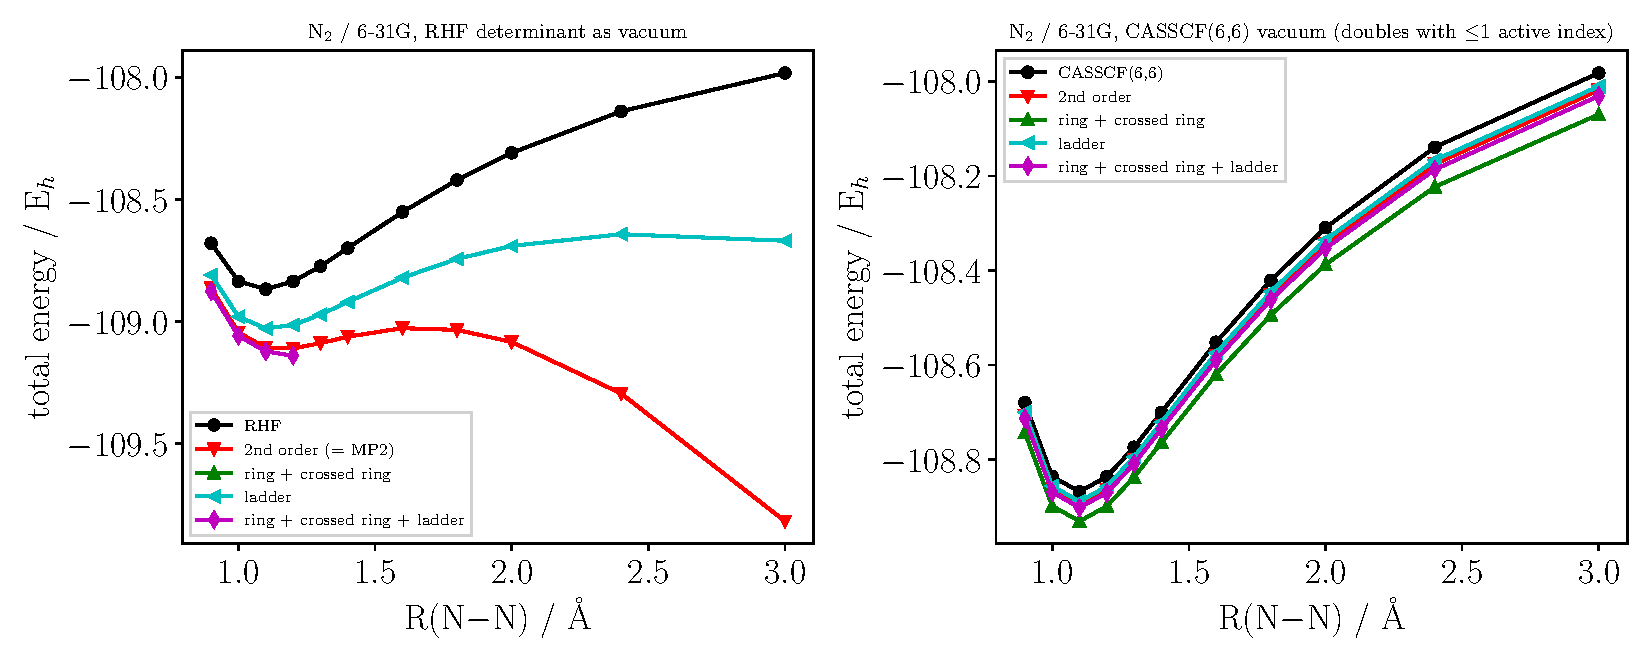
\includegraphics[width=0.95\textwidth]{erpa_ccd_n2_631g_totals.pdf}
\caption{N$_2$/6-31G total energies.  Left: RHF determinant as vacuum
(points are shown only where the iterations converged; the
ring$+$crossed-ring variant never does).  Right: CASSCF(6,6) vacuum with the
doubles with at most one active index, as in Table~\ref{tab:631g}.}
\label{fig:totals}
\end{figure*}

\subsection{Why the equations stop converging; the single-reference limit}
\label{sec:convergence}

Three diagnostics on the RHF reference separate two mechanisms
(\texttt{diag\_stability.py}, \texttt{diag\_linear.py}, \texttt{diag\_newton.py},
\texttt{diag\_mosaic.py}).

\emph{RPAx stability.}  Table~\ref{tab:stability} lists the lowest TDA
eigenvalue, the lowest eigenvalue of $\bA-\bB$ and the lowest RPAx frequency
of the RHF reference in 6-31G, and the same quantities for the external
ERPA manifold on the CASSCF(6,6) vacuum.  The RHF reference has its triplet
instability ($\bA-\bB$ indefinite, $\omega^2<0$) from $1.2$~\AA\ and
imaginary frequencies from $1.6$~\AA; the external ERPA problem on the
CASSCF vacuum never comes close to an instability (lowest frequency
$0.40$--$0.49$~E$_h$ along the curve), which is why every variant converges
there.

\begin{table}[t]
\caption{Stability indicators (E$_h$) for N$_2$/6-31G: RHF reference (all
$ij\to ab$ pairs) and external ERPA manifold on the CASSCF(6,6) vacuum
(pairs $ai$, $xi$, $ax$).  $n_-$ is the number of negative $\omega^2$.}
\label{tab:stability}
\begin{ruledtabular}
\begin{tabular}{cccccccc}
& \multicolumn{4}{c}{RHF} & \multicolumn{3}{c}{CASSCF(6,6), external}\\
$R$/\AA & min TDA & min$(\bA{-}\bB)$ & $\omega_{\min}$ & $n_-$ & min TDA & min$(\bA{-}\bB)$ & $\omega_{\min}$\\
\hline
0.90 & 0.417 & 0.242 & 0.385 & 0 & 0.494 & 0.421 & 0.486\\
1.00 & 0.314 & 0.120 & 0.246 & 0 & 0.465 & 0.392 & 0.457\\
1.10 & 0.219 & 0.021 & 0.093 & 0 & 0.445 & 0.372 & 0.436\\
1.20 & 0.142 & $-0.061$ & 0.092 & 3 & 0.433 & 0.361 & 0.425\\
1.30 & 0.077 & $-0.130$ & 0.087 & 9 & 0.429 & 0.358 & 0.421\\
1.40 & 0.023 & $-0.188$ & 0.079 & 13 & 0.432 & 0.363 & 0.425\\
1.60 & $-0.060$ & $-0.282$ & $0.027i$ & 29 & 0.458 & 0.395 & 0.452\\
2.00 & $-0.164$ & $-0.408$ & $0.104i$ & 35 & 0.431 & 0.432 & 0.424\\
3.00 & $-0.264$ & $-0.551$ & $0.059i$ & 35 & 0.401 & 0.410 & 0.396\\
\end{tabular}
\end{ruledtabular}
\end{table}

\emph{Linearized equations.}  The Jacobian of each variant at $\bt=0$,
preconditioned by the second-order denominators, has the following lowest
eigenvalues for N$_2$/STO-3G at $R=0.9$, $1.1$, $1.3$, $1.6$~\AA\ (each
threefold degenerate, \ie\ triplet coupled): ladder $1.04$, $1.03$, $1.03$,
$1.03$; full (non-mosaic CCD) $0.35$, $0.28$, $0.11$, $-0.21$;
ring$+$crossed ring $-0.12$, $-0.33$, $-0.65$, $-1.23$.  The full
linearization is the CISD doubles block $H_{DD}-E_0$ and stays positive up to
about $1.4$~\AA; the ring$+$crossed-ring linearization is the same block
\emph{without} the particle--particle and hole--hole ladder blocks and is
indefinite already at the equilibrium distance, where RPAx is perfectly
stable.  Newton--Krylov iterations started from the second-order amplitude
find no real solution of the ring$+$crossed-ring equation at $0.9$ and
$1.1$~\AA, while they reproduce the fixed-point solutions of the ladder and
full equations.  The failure of the ring$+$crossed-ring variant is therefore
not an RPA instability: once the ladders are dropped, the repulsive
Coulomb interaction of the two particles and of the two holes is missing
while the attractive exchange ring terms remain, and the doubles
``excitation energies'' of the linearized problem turn negative.  (The
single-channel RPAx Riccati equation, which is not antisymmetrized and whose
linearization is $\bA\otimes\bI+\bI\otimes\bA$, does have a solution there,
but an unphysically large one near the instability; it is the
antisymmetrized ring$+$crossed-ring combination that has none.)

\emph{Quadratic terms and the mosaic terms.}  The combined equation fails
from $1.3$~\AA\ although its linearization is still positive: the quadratic
ring term $\bN\bt\bB\bt\bN$ grows as the triplet instability is approached
and the Jacobian loses positivity along the iteration.  This is where the
analogy with CCD is instructive.  Full CCD differs from the non-mosaic
equation only by the two mosaic terms
$-\tfrac12P(ab)\sum\langle kl||cd\rangle t^{ac}_{ij}t^{bd}_{kl}-\tfrac12P(ij)\sum\langle kl||cd\rangle t^{ab}_{ik}t^{cd}_{jl}$,
which dress the one-body energies by the pair correlation (the
amplitude-space image of self-energy insertions, cf.\ \texttt{freqdepen\_eom.tex})
and belong to no channel.  With them added to the Hartree--Fock-limit
equation (Table~\ref{tab:mosaic}) the solution persists across the triplet
instability and follows CCSD to within a few mE$_h$; without them it does
not.  The coupling of the channels therefore does remove the single-channel
instability in the way CCD does, but only together with the mosaic terms;
the common-amplitude construction, which by design retains channel terms
only, inherits part of the single-channel fragility.  On the CASSCF vacuum
this does not matter for the external classes, because the external
problem is stable; it will matter if the construction is pushed to
references with strong external correlation (as in the $\sigma$-CAS(2,2)
test, where the ring-containing variants stop converging beyond $1.1$~\AA).

\begin{table}[t]
\caption{N$_2$/STO-3G on the RHF determinant: correlation energies (E$_h$)
of the non-mosaic equation \eqref{eq:combined}, of full CCD (mosaic terms
added), and of CCSD; the same fixed-point/DIIS solver for the first two;
n.c.\ = not converged.}
\label{tab:mosaic}
\begin{ruledtabular}
\begin{tabular}{ccccc}
$R$/\AA & $E_{\rm RHF}$/E$_h$ & non-mosaic CCD & full CCD & CCSD\\
\hline
0.90 & $-107.187190$ & $-0.11135$ & $-0.10406$ & $-0.10418$\\
1.10 & $-107.496501$ & $-0.17923$ & $-0.15346$ & $-0.15370$\\
1.30 & $-107.433871$ & n.c. & $-0.21654$ & $-0.21696$\\
1.60 & $-107.184846$ & n.c. & $-0.34378$ & $-0.34451$\\
2.00 & $-106.871504$ & n.c. & $-0.68220$ & $-0.68548$\\
2.40 & $-106.656608$ & n.c. & n.c. & n.c.\\
3.00 & $-106.479843$ & n.c. & $-1.16615$ & n.c.\\
\end{tabular}
\end{ruledtabular}
\end{table}

\subsection{Dependence on the size of the active space}
\label{sec:active-size}

Enlarging the active space moves correlation into the reference and changes
the composition of what is left outside (Table~\ref{tab:actsize};
\texttt{active\_space\_scan.py}).  Going from the CAS(6,6) of the $\sigma$ and
$\pi$ bonds to the full-valence CAS(10,8) lowers $E_{\rm CASSCF}$ by
$13$~mE$_h$ and the SC-NEVPT2 external correlation from $68$ to $58$~mE$_h$,
but the classes with at most one active index, the only ones the quasi-boson
construction treats correctly, collapse from $26$~mE$_h$ ($39\%$ of the
external correlation) to $0.9$~mE$_h$ ($1.5\%$), because the remaining core
is the $1s$ shell only.  The external correlation is then almost entirely of
the two-active-index type ($xy\to ab$, $31$~mE$_h$) and semi-internal
($27$~mE$_h$).  The channel variants on the one-active-index classes follow
this collapse (second order $-0.85$~mE$_h$, equal to the NEVPT2 value), the
external ERPA problem becomes even more stable (lowest frequency
$0.44\to0.89$~E$_h$), and the quasi-boson treatment of the two-active-index
doubles deteriorates further (norm ratios up to $290$ for the $1s^2\to xy$
doubles into the nearly filled $2s$-derived orbitals; its second order gives
$-207$~mE$_h$).  In the minimal basis the full-valence CAS(10,8) leaves only
$0.13$~mE$_h$ of core correlation outside the reference, which the
quasi-boson second order overestimates a hundredfold ($-12.6$~mE$_h$).  So a
larger active space makes the external problem smaller and better
conditioned, but it also removes the part of it that the quasi-boson
construction describes; the two-active-index and semi-internal classes, and
hence the pair-boson extension of Sec.~\ref{sec:validity}, become mandatory.

\begin{table}[t]
\caption{N$_2$/6-31G at $1.1$~\AA\ ($2.0$~\AA\ in parentheses), mE$_h$.
SC-NEVPT2 external correlation split into classes with one active index
($S_{ijrs},S_{ijr},S_{rsi}$), two active indices ($S_{ij},S_{rs}$) and the
semi-internal classes; channel variants on the one-active-index classes;
lowest external ERPA frequency (E$_h$); largest ratio of exact to quasi-boson
doubles norm in the $xy\to ab$ and $ij\to xy$ classes.}
\label{tab:actsize}
\begin{ruledtabular}
\begin{tabular}{lcc}
 & CAS(6,6) & CAS(10,8)\\
\hline
$E_{\rm CASSCF}$/E$_h$ & $-109.01594$ ($-108.77349$) & $-109.02919$ ($-108.77759$)\\
NEVPT2 total & $-67.8$ ($-65.4$) & $-58.1$ ($-60.5$)\\
\ \ one active index & $-26.3$ ($-33.5$) & $-0.9$ ($-1.2$)\\
\ \ two active indices & $-15.5$ ($-13.2$) & $-30.7$ ($-36.1$)\\
\ \ semi-internal & $-25.9$ ($-18.8$) & $-26.5$ ($-23.1$)\\
2nd order, one active index & $-27.0$ ($-33.3$) & $-0.9$ ($-1.2$)\\
ring$+$crossed ring & $-62.4$ ($-77.8$) & $-1.0$ ($-1.4$)\\
ladder & $-20.5$ ($-25.7$) & $-0.8$ ($-1.1$)\\
all three & $-33.6$ ($-43.7$) & $-0.9$ ($-1.2$)\\
$\omega_{\min}$, external ERPA & 0.44 (0.42) & 0.89 (0.91)\\
norm ratio, $xy\to ab$ & 32 (3.3) & 28 (3.4)\\
norm ratio, $ij\to xy$ & 32 (3.3) & 289 (683)\\
\end{tabular}
\end{ruledtabular}
\end{table}

%%%%%%%%%%%%%%%%%%%%%%%%%
\section{Conclusions}
\label{sec:conclusions}
%%%%%%%%%%%%%%%%%%%%%%%%%

\begin{enumerate}
\item The Pa2CCD construction extends to an arbitrary vacuum.  The channel
  Riccati equations are Eqs.~\eqref{eq:riccati-ph} and \eqref{eq:riccati-pp}
  with the ERPA metrics; the sources and free terms are no longer common and
  are replaced by their fermionic antisymmetrization; the result is
  Eq.~\eqref{eq:combined} on the external doubles space \eqref{eq:Dext}.  It
  reduces to non-mosaic CCD for a determinant.
\item The energy is the CCD-type functional \eqref{eq:Ec}, whose source is
  the exact coupling $\langle\Psi_0|\hat H|\Phi\rangle$ and whose second-order
  limit is the internally contracted second order with quasi-boson norms;
  for the classes with one active index it coincides with the SC-NEVPT2
  classes to within $0.4$~mE$_h$ per class.
\item Combining the channels does improve on the uncoupled channels where
  the construction applies: the ring channel alone (the ERPA correlation
  energy) overestimates by a factor $2$--$3$ or does not converge, the
  ladder channel alone recovers about half, and the combination is within
  $6$--$16\%$ of the exact-metric class energies and converges along the
  whole 6-31G curve.
\item The convergence failures on the RHF reference have two causes: the
  ring$+$crossed-ring equation without ladders has an indefinite linearization
  already at equilibrium (no real solution), and the combined equation loses
  its solution at the RHF triplet instability because the mosaic terms, which
  keep full CCD solvable there, are not channel terms.  On the CASSCF vacuum
  the external problem is stable along the whole curve.
\item The quasi-boson factorization of the doubles norm is exact only when
  one of the two excitations involves a core$\to$virtual boson.  For doubles
  with two active indices it replaces $1-n_x-n_y+\Gamma_{xy,xy}$ by
  $(1-n_x)(1-n_y)$, which fails by an order of magnitude for the nearly
  filled or empty natural orbitals of N$_2$ at equilibrium.  These are the
  only external doubles of the minimal-basis CAS(6,6) problem, so the STO-3G
  dissociation curve is not described by Eq.~\eqref{eq:combined}, whereas an
  exact-metric treatment of the same two classes recovers $98\%$ of
  $E_{\rm FCI}-E_{\rm CASSCF}$.  The consistent extension replaces the
  product of two $N{\pm}1$ bosons by one $N{\pm}2$ pair boson with the
  pair-EKT metric $\mathcal N^{\pm}$, which is available from the 2-RDM
  ($\mathcal N^{+}=S^{\pp}+\Gamma^{T}$) and is the natural particle--particle
  counterpart of the EKT charged states of \texttt{mr-hedin.tex}.  The
  semi-internal classes require the analogous three-index objects.
\end{enumerate}

%%%%%%%%%%%%%%%%%%%%%%%%
\bibliography{parquet-mr-hedin}
%%%%%%%%%%%%%%%%%%%%%%%%

\end{document}
